\section{MARCO REFERENCIAL}
\rule{\textwidth}{1pt}\\

Debe incluir la información pertinente para que el lector pueda realizar una lectura adecuada del documento, se recomienda subdividir en los marcos descriptivos que contextualicen al lector en los aspectos relevantes del proyecto (mínimo estado del arte y fundamentos teóricos, opcional marco legal, geogrífico, social, cultural, ambiental ...).
\subsection{ESTADO DEL ARTE}
Relacionar trabajos de otros autores relacionados con el trabajo que se desarrolla en esta investigación. Mostrar ventajas, desventajas, principios de operación y condiciones de operación de dichos trabajos.
\subsection{FUNDAMENTOS TEÓRICOS}
\subsubsection{Citas}
Es necesario soportar las afirmaciones y enunciados teóricos mediante referencias bibliográficas confiables (trabajos de grado, tesis de maestría, tesis de doctorado, artículos de revistas indexadas, artículos de ponencias, libros, notas de aplicación). Para la organización de las fuentes consultadas se recomienda usar un gestor de referencias bibliográficas: Mendeley, Docear, Zotero, etc.\\
En cuanto al estilo de citación, en esta plantilla se sugiere IEEE, por ser el estándar de nuestra área de conocimiento \cite{Chaparro}.
\subsubsection{Figuras y Tablas}
A continuación, un ejemplo de inserción de Figuras y Tablas:
En la Figura \ref{Fig: colectores de energia} se observa la clasificación de las fuentes y su principio de funcionamiento.
\begin{figure}[H]
	\centering
	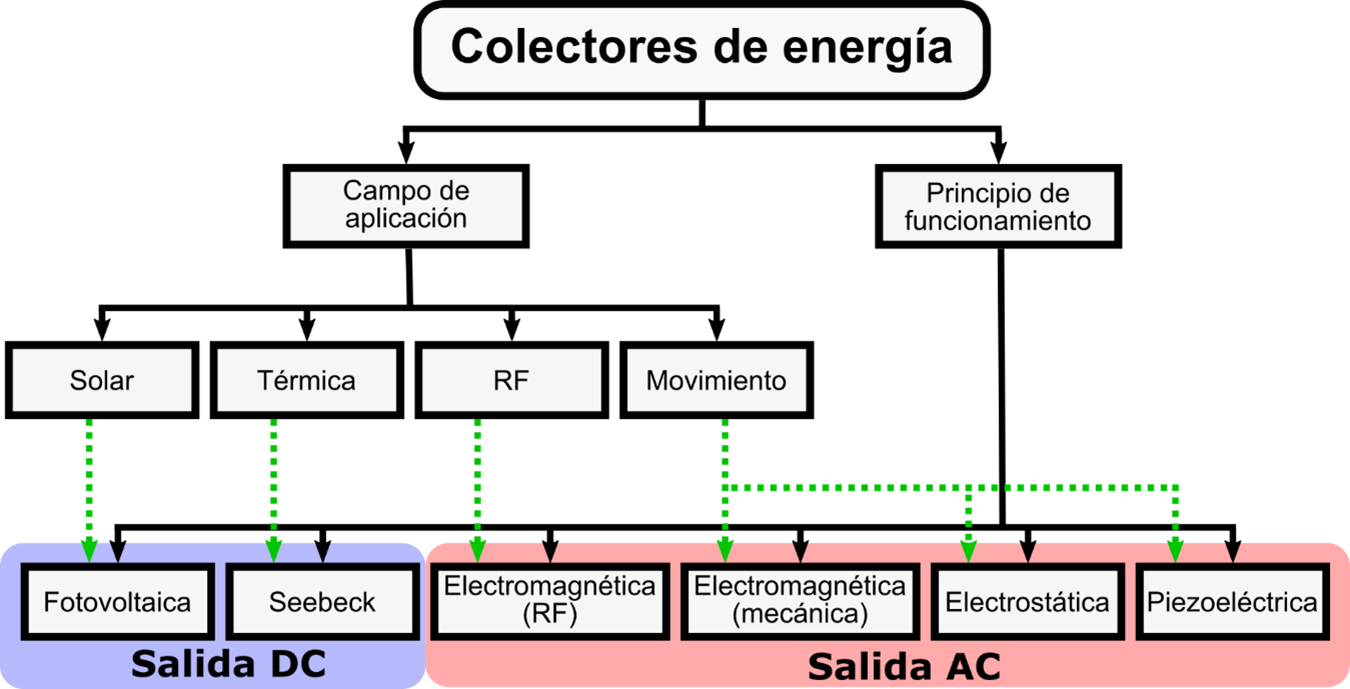
\includegraphics[width=0.9\textwidth]{energy_collectors}
	\caption{Recolectores de energia}
	\label{Fig: colectores de energia}
\end{figure}
En la Tabla \ref{Tab: fuentes de energia} se muestran las características resumidas de las diferentes fuentes analizadas.
\begin{table}[H]
	\centering
	\caption[Características de las fuentes de energía del entorno \cite{Rodriguez}.]{Principales características de las fuentes de energía del entorno \cite{Rodriguez}.}
	\label{Tab: fuentes de energia}
	\begin{tabular}{m{2.9cm}m{2.5cm}m{4.5cm}m{3.3cm}}
		\hline
		& \textbf{Solar PV} & \textbf{Termoeléctrica} &\textbf{Vibración piezoeléctrica} \\
		\hline
		\textbf{Densidad de potencia} & $100mW/cm^2$ & $50-100\mu W/cm^2$ \textit{por} $^{\circ} C$ & $10-200\mu W/cm^3$  \\
		\textbf{Tensión de salida} & $0.5V$ & $10-100mV$ & $10-20V$ \\
		\textbf{Condición de disponibilidad} & \textit{Ambiente iluminado} & \textit{Superficies} $\Delta T$ & \textit{Vibración Hz-KHz} \\
		\hline
	\end{tabular}
	\caption*{Nota:}
\end{table}
Como se observa, las tablas llevan su título en la parte superior y las figuras lo llevan en la parte inferior. De ser necesario puede colocar una nota al pie de la figura o tabla.\\

\textbf{IMPORTANTE PARA ESTA PLANTILLA:} Para esta plantilla en los caption de imagenes o tablas se recomienda usar la sigueinte sintaxis:
\begin{center}
	\small{\footnotesize }{\textit{$\backslash$caption[Caption que aparece en el indice de tablas o figuras]\{Caption para la figura o tabla\}}}
\end{center}
Se recomienda que el caption que aparece en el indice de tablas o figuras sea lo mas corto posible para evitar overlap entre los demás.
\newpage